\documentclass[12pt]{exam}

\usepackage{amssymb,amsfonts,amsmath}
\usepackage[letterpaper,margin=1in]{geometry}
\usepackage{graphicx}
\usepackage[numbered]{matlab-prettifier}
\usepackage{adjustbox}
\usepackage[T1]{fontenc}
\usepackage{mathtools}
\usepackage{color}
\usepackage{float}
\usepackage{bbold}

\DeclarePairedDelimiter{\abs}{\lvert}{\rvert}
\DeclarePairedDelimiter{\norm}{\lVert}{\rVert}

\renewcommand*{\vec}[1]{\boldsymbol{#1}}

\newcommand{\class}{Physics 306L}
\newcommand{\term}{Fall 2016}
\newcommand{\doctitle}{Lab Write-Up 11: Oscillators II}

\parindent 0ex

\pagestyle{head}
\header{\bf \class}{\bf \doctitle\ - Page \thepage\ of \numpages}{\bf \term}
\headrule


\begin{document}
\framebox{\parbox{\dimexpr\linewidth-2\fboxsep-2\fboxrule}{
\begin{centering}
\textbf{\underline{Relaxation Oscillator Values and Functions}}\\
$R_1 =47.75 k\Omega, \quad R_2 =47.47 k\Omega $\\
$R_3 \quad\text{values:}\quad 21.75k\Omega,\quad 6.778k\Omega,\quad2.199k\Omega,\quad.986k\Omega$\\
$\text{C values:}\quad 325\text{nF},\quad45\text{nF},\quad33.19\text{nF},\quad4.5\text{nF}$\\
\textbf{\underline{Function Used}}\\
$f=\frac{1}{R_3C},\quad f=\frac{1}{2(\text{ln}3)R_3C} $\\
\textbf{\underline{Measurement/Measured Data}}\\
F = 64.9 Hz, 1520 Hz, 85400 Hz, 272000 Hz\\
\textbf{Slew Rate:}  $1.92 \frac{\text{Volts}}{\mu\text{s}}$\\
\end{centering}
\begin{figure}[H]
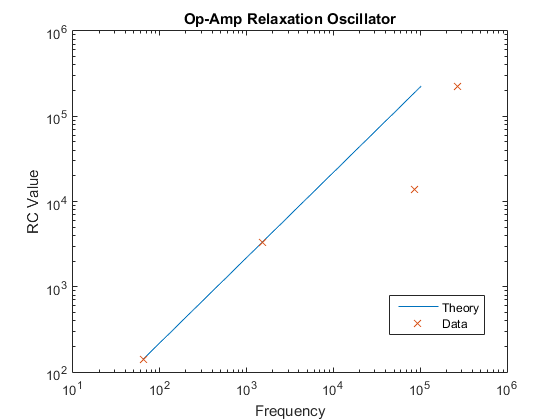
\includegraphics[width=\textwidth,keepaspectratio=true]{relaxation.png}
\end{figure}
}}


\framebox{\parbox{\dimexpr\linewidth-2\fboxsep-2\fboxrule}{
\begin{centering}
\textbf{\underline{555 Timer Values Part 1}}\\
$R_1 =.98 k\Omega$\\
$R_2 \quad\text{values:}\quad 21.75k\Omega,\quad 6.778k\Omega,\quad2.199k\Omega,\quad.986k\Omega$\\
C values:$\quad 325\text{nF},\quad45\text{nF},\quad33.19\text{nF},\quad4.5\text{nF}$\\
\textbf{555 Timer Values Part 2 (Duty Cycle)}\\
$R_2 =21.75 k\Omega$\\
$R_1 \quad\text{values:}\quad.98k\Omega,\quad 10k\Omega,\quad47.41k\Omega,\quad400k\Omega$\\
C = 3.256nF\\
\textbf{\underline{Function Used}}\\
$f= \frac{1}{R_3C},\quad f = \frac{1.44}{(R_1 + 2R_2)C},\quad \text{DC} = \frac{R_1 + R_2}{R_1 + 2R_2}$\\
\textbf{\underline{Measurement/Measured Data}}\\
F = 64.9 Hz, 1520 Hz, 85400 Hz, 272000 Hz\\
DC = 50\%, 63\%, 81\%, 95\%\\
\end{centering}
\begin{figure}[H]
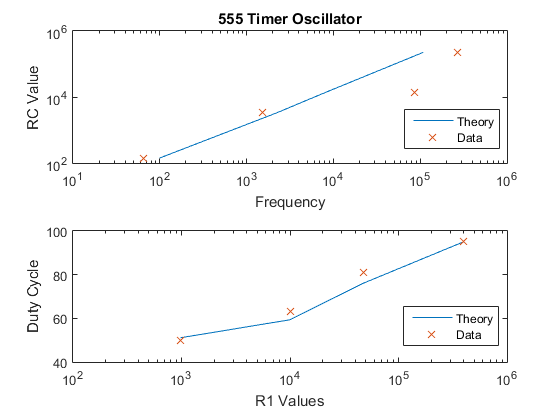
\includegraphics[width=\textwidth,keepaspectratio=true]{timer.png}
\end{figure}
}}


\framebox{\parbox{\dimexpr\linewidth-2\fboxsep-2\fboxrule}{
\begin{centering}
\textbf{\underline{555 VCO}}\\
$R_1 = 47 k\Omega,\quad R_2= 47.3k\Omega$\\
C = 9.8 nF\\
\textbf{\underline{Measurement/Measured Data}}\\
Voltage Values: .5 V, 1.5 V, 2.5 V, 3.5 V, 4.5 V\\
Frequency: 2599.069 Hz, 2000.003 Hz, 1421.25 Hz, 950.05 Hz, 518.607 Hz\\
DC: 15\%, 35\%, 55\%, 70\%, 88\%\\
\end{centering}

\begin{figure}[H]
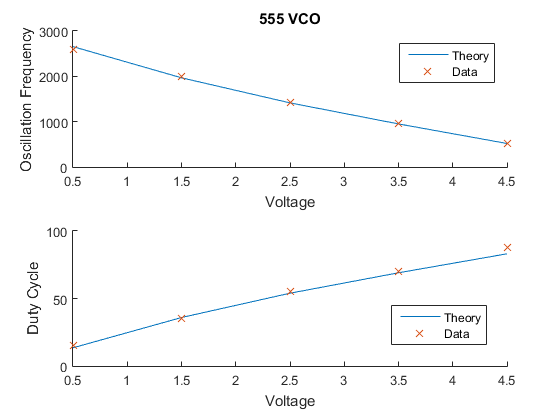
\includegraphics[width=\textwidth,keepaspectratio=true]{vco.png}
\end{figure}
}}


\end{document}
